
\documentclass[aspectratio=169,11pt]{beamer}

% ---------- Theme & typography ----------
\usetheme{Madrid}
\usecolortheme{default}
\usefonttheme{professionalfonts}
\setbeamertemplate{navigation symbols}{}
\setbeamertemplate{footline}{
  \leavevmode%
  \hbox{
    \begin{beamercolorbox}[wd=.78\paperwidth,ht=2.5ex,dp=1ex,leftskip=1em]{author in head/foot}
      \color{gray!80}\small CUSAT M.Tech AI \& Software Engineering \quad|\quad Linear Algebra
    \end{beamercolorbox}%
    \begin{beamercolorbox}[wd=.22\paperwidth,ht=2.5ex,dp=1ex,rightskip=1em]{date in head/foot}
      \hfill\color{gray!80}\small \insertframenumber/\inserttotalframenumber
    \end{beamercolorbox}}
}

\definecolor{cusatblue}{RGB}{20,66,114}
\definecolor{deepblue}{RGB}{12,39,70}
\definecolor{teal}{RGB}{0,121,140}
\definecolor{softblue}{RGB}{232,242,250}
\definecolor{softteal}{RGB}{231,247,247}
\definecolor{softgold}{RGB}{250,246,226}
\definecolor{darkgray}{RGB}{55,62,70}

\setbeamercolor{structure}{fg=cusatblue}
\setbeamercolor{frametitle}{fg=white,bg=cusatblue}
\setbeamercolor{title}{fg=deepblue}
\setbeamercolor{subtitle}{fg=teal}
\setbeamercolor{normal text}{fg=darkgray}
\setbeamercolor{block title}{fg=white,bg=cusatblue}
\setbeamercolor{block body}{fg=darkgray,bg=softblue}
\setbeamercolor{alertblock title}{fg=white,bg=teal}
\setbeamercolor{alertblock body}{fg=darkgray,bg=softteal}
\setbeamercolor{exampleblock title}{fg=white,bg=deepblue}
\setbeamercolor{exampleblock body}{fg=darkgray,bg=softgold}

\setbeamertemplate{itemize item}{\color{teal}$\blacktriangleright$}
\setbeamertemplate{itemize subitem}{\color{cusatblue}$\bullet$}
\setlength{\parskip}{4pt}

\usepackage{amsmath,amssymb,bm,mathtools}
\usepackage{booktabs,array}
\usepackage{tikz}
\usetikzlibrary{arrows.meta,positioning,calc,decorations.pathreplacing}
\usepackage{tcolorbox}
\usepackage{hyperref}
\hypersetup{colorlinks=true,linkcolor=cusatblue,urlcolor=teal}

\newcommand{\R}{\mathbb{R}}
\newcommand{\vect}[1]{\bm{#1}}
\newcommand{\T}{^{\mathsf T}}
\newcommand{\important}[1]{\textcolor{teal}{\textbf{#1}}}

% ---------- Title ----------
\title{\textbf{Linear Algebra}}
\subtitle{CUSAT M.Tech. Computer Science \& Engineering\\Artificial Intelligence \& Software Engineering}
\author{Sayona C. Sajan}
\institute{Cochin University of Science and Technology}
\date{September 2026}

\begin{document}

% ============================================================
\begin{frame}
  \titlepage
  \vspace{-0.4cm}
  \begin{center}
    \small\color{gray}
    Vectors $\rightarrow$ Transformations $\rightarrow$ Subspaces $\rightarrow$
    Eigenstructure
  \end{center}
\end{frame}

\begin{frame}{Why Linear Algebra matters in AI \& Software Engineering}
\begin{columns}[T]
\column{0.48\textwidth}
\begin{block}{Core idea}
Linear algebra gives a language for representing data, transformations and constraints.
\end{block}
\begin{itemize}
\item Data points and features $\rightarrow$ vectors
\item Neural-network layers $\rightarrow$ matrix transformations
\item Similarity $\rightarrow$ dot products
\item Geometry $\rightarrow$ transformations and cross products
\item Stable directions $\rightarrow$ eigenvectors
\end{itemize}
\column{0.48\textwidth}
\begin{exampleblock}{Exam mindset}
For every topic ask:
\begin{enumerate}
\item What is the definition?
\item What is the geometric meaning?
\item What is the formula?
\item Can I compute a small example?
\item What changes in higher dimensions?
\end{enumerate}
\end{exampleblock}
\end{columns}
\end{frame}

\begin{frame}{Syllabus map}
\begin{center}
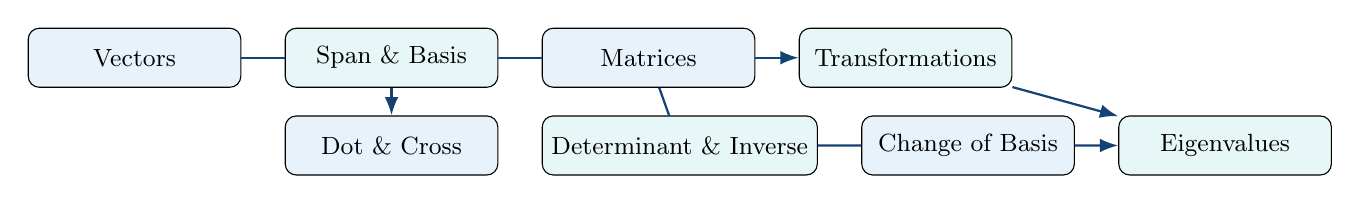
\begin{tikzpicture}[node distance=0.35cm and 0.55cm, every node/.style={font=\small}]
\node[draw,rounded corners,fill=softblue,minimum width=2.7cm,minimum height=.75cm] (v) {Vectors};
\node[draw,rounded corners,fill=softteal,minimum width=2.7cm,minimum height=.75cm,right=of v] (s) {Span \& Basis};
\node[draw,rounded corners,fill=softblue,minimum width=2.7cm,minimum height=.75cm,right=of s] (m) {Matrices};
\node[draw,rounded corners,fill=softteal,minimum width=2.7cm,minimum height=.75cm,right=of m] (t) {Transformations};
\node[draw,rounded corners,fill=softblue,minimum width=2.7cm,minimum height=.75cm,below=of s] (d) {Dot \& Cross};
\node[draw,rounded corners,fill=softteal,minimum width=2.7cm,minimum height=.75cm,right=of d] (e) {Determinant \& Inverse};
\node[draw,rounded corners,fill=softblue,minimum width=2.7cm,minimum height=.75cm,right=of e] (c) {Change of Basis};
\node[draw,rounded corners,fill=softteal,minimum width=2.7cm,minimum height=.75cm,right=of c] (ev) {Eigenvalues};
\draw[-{Latex},thick,cusatblue] (v)--(s)--(m)--(t);
\draw[-{Latex},thick,cusatblue] (s)--(d);
\draw[-{Latex},thick,cusatblue] (m)--(e)--(c)--(ev);
\draw[-{Latex},thick,cusatblue] (t)--(ev);
\end{tikzpicture}
\end{center}
\vspace{.3cm}
\begin{alertblock}{Coverage}
This deck follows the supplied CUSAT Linear Algebra syllabus and emphasizes definitions, intuition, derivations, computations, and exam-style checks.
\end{alertblock}
\end{frame}

% ============================================================
\section{Vectors and Coordinate Systems}
\begin{frame}{1. Vectors and coordinate systems}
A vector has both \important{magnitude} and \important{direction}.
\[
\vect v=
\begin{bmatrix}v_1\\v_2\\v_3\end{bmatrix}
=v_1\vect e_1+v_2\vect e_2+v_3\vect e_3
\]
where
\[
\vect e_1=\begin{bmatrix}1\\0\\0\end{bmatrix},\quad
\vect e_2=\begin{bmatrix}0\\1\\0\end{bmatrix},\quad
\vect e_3=\begin{bmatrix}0\\0\\1\end{bmatrix}.
\]
\begin{itemize}
\item $\R^2$: ordered pairs $(x,y)$
\item $\R^3$: ordered triples $(x,y,z)$
\item The origin is the zero vector.
\item Coordinates depend on the chosen basis.
\end{itemize}
\end{frame}

\begin{frame}{Vector addition and scalar multiplication}
For
\[
\vect u=\begin{bmatrix}u_1\\u_2\\u_3\end{bmatrix},\qquad
\vect v=\begin{bmatrix}v_1\\v_2\\v_3\end{bmatrix},
\]
\[
\vect u+\vect v=
\begin{bmatrix}
u_1+v_1\\u_2+v_2\\u_3+v_3
\end{bmatrix},
\qquad
c\vect u=
\begin{bmatrix}
cu_1\\cu_2\\cu_3
\end{bmatrix}.
\]
\begin{exampleblock}{Example}
\[
\begin{bmatrix}1\\2\\-1\end{bmatrix}
+2\begin{bmatrix}3\\0\\4\end{bmatrix}
=
\begin{bmatrix}7\\2\\7\end{bmatrix}.
\]
\end{exampleblock}
\begin{center}
\textbf{Think geometrically:} addition translates one arrow; scalar multiplication stretches, shrinks, or reverses it.
\end{center}
\end{frame}

\begin{frame}{Linear combinations}
A \important{linear combination} of $\vect v_1,\ldots,\vect v_k$ is
\[
c_1\vect v_1+c_2\vect v_2+\cdots+c_k\vect v_k.
\]
\begin{block}{Key question}
Can a target vector $\vect b$ be written as a linear combination of the given vectors?
\[
A\vect x=\vect b
\]
is exactly the coefficient-finding problem.
\end{block}
\begin{exampleblock}{Example}
\[
2\begin{bmatrix}1\\0\end{bmatrix}
-3\begin{bmatrix}0\\1\end{bmatrix}
=
\begin{bmatrix}2\\-3\end{bmatrix}.
\]
Thus every vector in $\R^2$ is a linear combination of the standard basis vectors.
\end{exampleblock}
\end{frame}

% ============================================================
\section{Span and Basis}
\begin{frame}{2. Span}
The \important{span} of vectors $\{\vect v_1,\ldots,\vect v_k\}$ is the set
\[
\operatorname{span}\{\vect v_1,\ldots,\vect v_k\}
=
\left\{
\sum_{i=1}^{k}c_i\vect v_i:c_i\in\R
\right\}.
\]
\begin{itemize}
\item One nonzero vector in $\R^2$ spans a line through the origin.
\item Two independent vectors in $\R^2$ span the whole plane.
\item Three independent vectors in $\R^3$ span all of $\R^3$.
\end{itemize}
\begin{alertblock}{Exam test}
To determine whether $\vect b$ lies in a span, solve $A\vect x=\vect b$.
\end{alertblock}
\end{frame}

\begin{frame}{Basis and dimension}
A set $B=\{\vect v_1,\ldots,\vect v_n\}$ is a \important{basis} if it is:
\begin{enumerate}
\item spanning, and
\item linearly independent.
\end{enumerate}
The number of basis vectors is the \important{dimension}.
\[
\dim(\R^n)=n.
\]
\begin{exampleblock}{Standard basis of $\R^3$}
\[
\left\{
\begin{bmatrix}1\\0\\0\end{bmatrix},
\begin{bmatrix}0\\1\\0\end{bmatrix},
\begin{bmatrix}0\\0\\1\end{bmatrix}
\right\}.
\]
\end{exampleblock}
\begin{block}{Important equivalence in $\R^n$}
For $n$ vectors: independent $\Longleftrightarrow$ spanning $\Longleftrightarrow$ basis.
\end{block}
\end{frame}

% ============================================================
\section{Matrices and Transformations}
\begin{frame}{3. Matrix multiplication as composition}
If
\[
T(\vect x)=A\vect x,\qquad S(\vect x)=B\vect x,
\]
then applying $T$ first and $S$ second gives
\[
S(T(\vect x))=B(A\vect x)=(BA)\vect x.
\]
\begin{alertblock}{Order matters}
\[
BA\neq AB\quad\text{in general.}
\]
Matrix multiplication represents composition of transformations, so the rightmost matrix acts first.
\end{alertblock}
\begin{exampleblock}{Mental model}
\[
\vect x \xrightarrow{\;A\;} A\vect x
\xrightarrow{\;B\;} BA\vect x.
\]
\end{exampleblock}
\end{frame}

\begin{frame}{Matrix multiplication: row $\times$ column}
For compatible matrices $A$ and $B$,
\[
(AB)_{ij}=\sum_k a_{ik}b_{kj}.
\]
\begin{exampleblock}{Example}
\[
\begin{bmatrix}1&2\\3&4\end{bmatrix}
\begin{bmatrix}5&6\\7&8\end{bmatrix}
=
\begin{bmatrix}
1(5)+2(7)&1(6)+2(8)\\
3(5)+4(7)&3(6)+4(8)
\end{bmatrix}
=
\begin{bmatrix}19&22\\43&50\end{bmatrix}.
\]
\end{exampleblock}
\begin{block}{Dimension rule}
$(m\times n)(n\times p)=(m\times p)$.
\end{block}
\end{frame}

\begin{frame}{Three-dimensional linear transformations}
A linear transformation $T:\R^3\to\R^3$ satisfies
\[
T(\vect u+\vect v)=T(\vect u)+T(\vect v),\qquad
T(c\vect u)=cT(\vect u).
\]
A $3\times3$ matrix acts on $\R^3$.
\begin{columns}[T]
\column{.5\textwidth}
\begin{itemize}
\item Scaling
\item Reflection
\item Rotation
\item Shearing
\item Projection
\end{itemize}
\column{.48\textwidth}
\begin{exampleblock}{Columns reveal the map}
If $A=[\vect a_1\ \vect a_2\ \vect a_3]$, then
\[
A\vect e_1=\vect a_1,\quad
A\vect e_2=\vect a_2,\quad
A\vect e_3=\vect a_3.
\]
\end{exampleblock}
\end{columns}
\end{frame}

\begin{frame}{Common 3D transformation matrices}
\small
\begin{columns}[T]
\column{.48\textwidth}
\textbf{Scaling}
\[
S=
\begin{bmatrix}
s_x&0&0\\0&s_y&0\\0&0&s_z
\end{bmatrix}
\]
\textbf{Rotation about $z$}
\[
R_z(\theta)=
\begin{bmatrix}
\cos\theta&-\sin\theta&0\\
\sin\theta&\cos\theta&0\\
0&0&1
\end{bmatrix}
\]
\column{.48\textwidth}
\textbf{Reflection in $xy$-plane}
\[
F=
\begin{bmatrix}
1&0&0\\0&1&0\\0&0&-1
\end{bmatrix}
\]
\textbf{Projection onto $xy$-plane}
\[
P=
\begin{bmatrix}
1&0&0\\0&1&0\\0&0&0
\end{bmatrix}
\]
\end{columns}
\end{frame}

% ============================================================
\section{Determinants and Inverses}
\begin{frame}{4. Determinant}
For
\[
A=\begin{bmatrix}a&b\\c&d\end{bmatrix},
\qquad
\det(A)=ad-bc.
\]
Geometrically, $|\det A|$ is the \important{area/volume scaling factor}.
\begin{itemize}
\item $\det(A)>0$: orientation preserved.
\item $\det(A)<0$: orientation reversed.
\item $\det(A)=0$: space is collapsed into a lower dimension.
\end{itemize}
\begin{alertblock}{Critical exam fact}
\[
\det(A)=0\quad\Longleftrightarrow\quad A\text{ is singular}.
\]
\end{alertblock}
\end{frame}

\begin{frame}{Determinant of a $3\times3$ matrix}
For
\[
A=
\begin{bmatrix}
a&b&c\\d&e&f\\g&h&i
\end{bmatrix},
\]
\[
\det(A)=
a(ei-fh)-b(di-fg)+c(dh-eg).
\]
\begin{exampleblock}{Fast method}
Expand along a row/column with zeros whenever possible. For hand calculations, keep the alternating signs:
\[
+\quad-\quad+.
\]
\end{exampleblock}
\begin{block}{Transformation viewpoint}
If $|\det A|=3$, every volume is multiplied by $3$ under $A$.
\end{block}
\end{frame}

\begin{frame}{Inverse matrices}
An inverse $A^{-1}$ satisfies
\[
AA^{-1}=A^{-1}A=I.
\]
For a $2\times2$ matrix,
\[
A^{-1}=
\frac{1}{ad-bc}
\begin{bmatrix}
d&-b\\-c&a
\end{bmatrix},
\qquad \det(A)\neq0.
\]
\begin{itemize}
\item $A^{-1}$ exists iff $\det(A)\neq0$ for a square matrix.
\item Solving $A\vect x=\vect b$:
\[
\vect x=A^{-1}\vect b.
\]
\item Numerically, Gaussian elimination is usually preferable to explicitly computing $A^{-1}$.
\end{itemize}
\end{frame}

% ============================================================
\section{Column Space and Null Space}
\begin{frame}{5. Column space}
For $A=[\vect a_1\ \cdots\ \vect a_n]$,
\[
\operatorname{Col}(A)=\operatorname{span}\{\vect a_1,\ldots,\vect a_n\}.
\]
It is the set of all possible outputs:
\[
\operatorname{Col}(A)=\{A\vect x:\vect x\in\R^n\}.
\]
\begin{block}{Connection to systems}
$A\vect x=\vect b$ has a solution exactly when
\[
\vect b\in\operatorname{Col}(A).
\]
\end{block}
\end{frame}

\begin{frame}{Null space}
The null space is
\[
\operatorname{Null}(A)=\{\vect x:A\vect x=\vect0\}.
\]
It contains every input that gets mapped to zero.
\begin{exampleblock}{Example}
\[
A=
\begin{bmatrix}1&2\\2&4\end{bmatrix}.
\]
Then
\[
x+2y=0\quad\Rightarrow\quad
\vect x=t\begin{bmatrix}-2\\1\end{bmatrix}.
\]
Hence
\[
\operatorname{Null}(A)=
\operatorname{span}\left\{
\begin{bmatrix}-2\\1\end{bmatrix}\right\}.
\]
\end{exampleblock}
\end{frame}

\begin{frame}{Rank--nullity connection}
For an $m\times n$ matrix $A$,
\[
\boxed{\operatorname{rank}(A)+\operatorname{nullity}(A)=n.}
\]
Here $n$ is the number of columns.
\begin{itemize}
\item $\operatorname{rank}(A)=\dim(\operatorname{Col}(A))$
\item $\operatorname{nullity}(A)=\dim(\operatorname{Null}(A))$
\end{itemize}
\begin{alertblock}{Exam shortcut}
Row-reduce $A$:
\[
\text{number of pivots}=\operatorname{rank}(A),
\quad
n-\text{number of pivots}=\operatorname{nullity}(A).
\]
\end{alertblock}
\end{frame}

% ============================================================
\section{Nonsquare Matrices}
\begin{frame}{6. Nonsquare matrices as transformations}
A matrix
\[
A\in\R^{m\times n}
\]
defines
\[
T:\R^n\to\R^m,\qquad T(\vect x)=A\vect x.
\]
\begin{center}
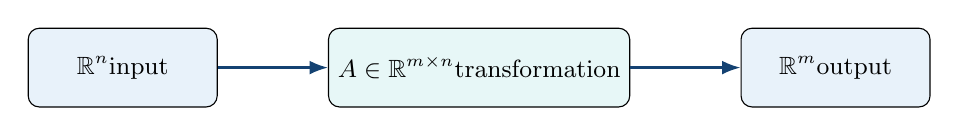
\begin{tikzpicture}[node distance=1.4cm, every node/.style={font=\small}]
\node[draw,rounded corners,fill=softblue,minimum width=2.4cm,minimum height=1cm] (a) {$\R^n$\\input};
\node[draw,rounded corners,fill=softteal,minimum width=2.7cm,minimum height=1cm,right=of a] (b) {$A\in\R^{m\times n}$\\transformation};
\node[draw,rounded corners,fill=softblue,minimum width=2.4cm,minimum height=1cm,right=of b] (c) {$\R^m$\\output};
\draw[-{Latex},thick,cusatblue] (a)--(b);
\draw[-{Latex},thick,cusatblue] (b)--(c);
\end{tikzpicture}
\end{center}
\begin{exampleblock}{Example}
A $2\times3$ matrix maps a 3D vector to a 2D vector:
\[
\R^3\longrightarrow\R^2.
\]
\end{exampleblock}
\end{frame}

% ============================================================
\section{Dot Products and Duality}
\begin{frame}{7. Dot product}
For $\vect u,\vect v\in\R^n$,
\[
\boxed{\vect u\cdot\vect v=\vect u\T\vect v
=\sum_{i=1}^n u_iv_i.}
\]
Geometrically,
\[
\vect u\cdot\vect v
=\|\vect u\|\,\|\vect v\|\cos\theta.
\]
\begin{itemize}
\item Positive $\Rightarrow$ acute angle.
\item Zero $\Rightarrow$ perpendicular.
\item Negative $\Rightarrow$ obtuse angle.
\end{itemize}
\begin{exampleblock}{Projection}
Projection of $\vect u$ onto $\vect v$:
\[
\operatorname{proj}_{\vect v}\vect u
=
\frac{\vect u\cdot\vect v}{\vect v\cdot\vect v}\vect v.
\]
\end{exampleblock}
\end{frame}

\begin{frame}{Duality: vectors as linear functionals}
A vector $\vect a$ can define a linear functional
\[
f_{\vect a}(\vect x)=\vect a\T\vect x.
\]
Thus the dot product converts a vector into a rule that maps vectors to scalars:
\[
\R^n\longrightarrow\R.
\]
\begin{block}{Why this matters}
The \important{dual space} consists of linear functionals. In Euclidean spaces, the dot product provides a natural correspondence between vectors and these functionals.
\end{block}
\begin{exampleblock}{Machine-learning connection}
A neuron's weighted sum is
\[
z=\vect w\T\vect x+b,
\]
a linear functional plus a bias.
\end{exampleblock}
\end{frame}

% ============================================================
\section{Cross Products}
\begin{frame}{8. Cross product in $\R^3$}
For
\[
\vect u=\begin{bmatrix}u_1\\u_2\\u_3\end{bmatrix},
\quad
\vect v=\begin{bmatrix}v_1\\v_2\\v_3\end{bmatrix},
\]
\[
\vect u\times\vect v=
\begin{bmatrix}
u_2v_3-u_3v_2\\
u_3v_1-u_1v_3\\
u_1v_2-u_2v_1
\end{bmatrix}.
\]
Properties:
\[
\vect u\times\vect v=-(\vect v\times\vect u),
\qquad
\vect u\times\vect v\perp\vect u,\vect v.
\]
Magnitude:
\[
\|\vect u\times\vect v\|
=\|\vect u\|\,\|\vect v\|\sin\theta.
\]
\end{frame}

\begin{frame}{Cross product and area}
The parallelogram generated by $\vect u,\vect v$ has area
\[
A=\|\vect u\times\vect v\|.
\]
The triangle has area
\[
A_{\triangle}=\frac12\|\vect u\times\vect v\|.
\]
\begin{exampleblock}{Quick example}
\[
\vect u=(1,0,0),\qquad\vect v=(0,2,0)
\]
gives
\[
\vect u\times\vect v=(0,0,2).
\]
So the parallelogram area is $2$.
\end{exampleblock}
\end{frame}

\begin{frame}{Cross products through linear transformations}
For an invertible $3\times3$ matrix $A$,
\[
\boxed{(A\vect u)\times(A\vect v)
=\det(A)\,A^{-\mathsf T}(\vect u\times\vect v).}
\]
This explains why the cross product transforms differently from an ordinary vector under a general linear transformation.
\begin{block}{Special case: rotation}
If $R$ is a proper rotation,
\[
\det(R)=1,\qquad R^{-\mathsf T}=R,
\]
so
\[
(R\vect u)\times(R\vect v)=R(\vect u\times\vect v).
\]
\end{block}
\end{frame}

% ============================================================
\section{Cramer's Rule}
\begin{frame}{9. Cramer's rule}
For a square system
\[
A\vect x=\vect b,\qquad \det(A)\neq0,
\]
the $i$th variable is
\[
\boxed{x_i=\frac{\det(A_i)}{\det(A)}}
\]
where $A_i$ is obtained by replacing column $i$ of $A$ with $\vect b$.
\begin{exampleblock}{For two variables}
\[
\begin{cases}
a_1x+b_1y=c_1\\
a_2x+b_2y=c_2
\end{cases}
\]
\[
x=\frac{\begin{vmatrix}c_1&b_1\\c_2&b_2\end{vmatrix}}
{\begin{vmatrix}a_1&b_1\\a_2&b_2\end{vmatrix}},
\quad
y=\frac{\begin{vmatrix}a_1&c_1\\a_2&c_2\end{vmatrix}}
{\begin{vmatrix}a_1&b_1\\a_2&b_2\end{vmatrix}}.
\]
\end{exampleblock}
\end{frame}

\begin{frame}{Cramer's rule: exam caution}
\begin{itemize}
\item Requires a \important{square} system.
\item Requires $\det(A)\neq0$ for a unique solution.
\item Elegant for small systems.
\item Usually inefficient for large numerical systems compared with elimination.
\end{itemize}
\begin{alertblock}{Do not confuse}
Cramer's rule is a formula for solving a system; it is not the same as Gaussian elimination.
\end{alertblock}
\end{frame}

% ============================================================
\section{Change of Basis}
\begin{frame}{10. Change of basis}
Suppose $B=\{\vect b_1,\ldots,\vect b_n\}$ is a basis. The coordinate vector of $\vect x$ in basis $B$ is
\[
[\vect x]_B=
\begin{bmatrix}c_1\\\vdots\\c_n\end{bmatrix}
\quad\text{where}\quad
\vect x=c_1\vect b_1+\cdots+c_n\vect b_n.
\]
Construct the basis matrix
\[
P_B=[\vect b_1\ \vect b_2\ \cdots\ \vect b_n].
\]
Then
\[
\boxed{\vect x=P_B[\vect x]_B}
\]
and
\[
\boxed{[\vect x]_B=P_B^{-1}\vect x}.
\]
\end{frame}

\begin{frame}{Change of basis between two bases}
Let $B$ and $C$ be bases. Then
\[
[\vect x]_C=P_C^{-1}P_B[\vect x]_B.
\]
The matrix
\[
P_{C\leftarrow B}=P_C^{-1}P_B
\]
converts coordinates from $B$ to $C$.
\begin{block}{Key idea}
The physical vector $\vect x$ does not change. Only its \important{coordinate description} changes.
\end{block}
\begin{exampleblock}{Exam question}
Given two bases and a vector, find $[\vect x]_B$, $[\vect x]_C$, or the transition matrix.
\end{exampleblock}
\end{frame}

% ============================================================
\section{Eigenvalues and Eigenvectors}
\begin{frame}{11. Eigenvectors and eigenvalues}
A nonzero vector $\vect v$ is an eigenvector of $A$ if
\[
A\vect v=\lambda\vect v.
\]
Here $\lambda$ is the corresponding eigenvalue.
Rearrange:
\[
(A-\lambda I)\vect v=\vect0.
\]
For a nonzero solution,
\[
\boxed{\det(A-\lambda I)=0.}
\]
This equation is the \important{characteristic equation}.
\end{frame}

\begin{frame}{How to find eigenvalues and eigenvectors}
\begin{enumerate}
\item Compute $A-\lambda I$.
\item Set $\det(A-\lambda I)=0$.
\item Solve for eigenvalues $\lambda$.
\item For each $\lambda$, solve
\[
(A-\lambda I)\vect v=\vect0.
\]
\item Give the eigenspace as the span of the eigenvectors.
\end{enumerate}
\begin{alertblock}{Important}
An eigenvector can never be the zero vector.
\end{alertblock}
\end{frame}

\begin{frame}{Geometric meaning of eigenvectors}
Most vectors change both direction and magnitude under a transformation.
An eigenvector changes only by a scalar:
\[
\vect v\longmapsto \lambda\vect v.
\]
\begin{itemize}
\item $|\lambda|>1$: stretching
\item $0<|\lambda|<1$: shrinking
\item $\lambda<0$: direction reversal
\item $\lambda=1$: unchanged
\item $\lambda=0$: mapped to zero
\end{itemize}
\begin{block}{AI connection}
Eigenvectors appear in PCA, spectral methods, covariance analysis, graph algorithms and dynamical systems.
\end{block}
\end{frame}

% ============================================================
\section{Vector Spaces}
\begin{frame}{12. Vector spaces}
A vector space over $\R$ is a set $V$ with vector addition and scalar multiplication satisfying the vector-space axioms.
Typical examples:
\[
\R^n,\quad
\text{polynomials},\quad
\text{matrices},\quad
\text{functions}.
\]
A subset $W\subseteq V$ is a subspace if:
\begin{enumerate}
\item $\vect0\in W$,
\item $\vect u,\vect v\in W\Rightarrow\vect u+\vect v\in W$,
\item $\vect u\in W,\ c\in\R\Rightarrow c\vect u\in W$.
\end{enumerate}
\end{frame}

\begin{frame}{Subspaces you should recognize}
For an $m\times n$ matrix $A$:
\[
\operatorname{Col}(A)\subseteq\R^m,\qquad
\operatorname{Null}(A)\subseteq\R^n.
\]
Both are vector spaces.
\begin{columns}[T]
\column{.48\textwidth}
\begin{block}{Column space}
All possible outputs $A\vect x$.
\end{block}
\column{.48\textwidth}
\begin{block}{Null space}
All inputs mapped to $\vect0$.
\end{block}
\end{columns}
\vspace{.2cm}
\[
\operatorname{rank}(A)=\dim\operatorname{Col}(A),\qquad
\operatorname{nullity}(A)=\dim\operatorname{Null}(A).
\]
\end{frame}

% ============================================================
\section{Integrated Problem Solving}
\begin{frame}{13. A complete exam workflow}
\begin{enumerate}
\item \textbf{Identify the object:} vector, matrix, transformation, subspace.
\item \textbf{Check dimensions:} especially before multiplication.
\item \textbf{Translate to equations:} e.g. $A\vect x=\vect b$.
\item \textbf{Choose the tool:} elimination, determinant, inverse, eigen-equation, dot/cross product.
\item \textbf{Interpret the answer geometrically.}
\item \textbf{Check}: dimensions, signs, determinant, substitution.
\end{enumerate}
\begin{alertblock}{CUSAT-style preparation}
Do not memorize formulas alone. Practice short numerical problems where the same concept appears in a different form.
\end{alertblock}
\end{frame}

\begin{frame}{High-yield formula sheet}
\small
\begin{align*}
\vect u\cdot\vect v&=\vect u\T\vect v
=\|\vect u\|\|\vect v\|\cos\theta\\
\operatorname{proj}_{\vect v}\vect u
&=\frac{\vect u\cdot\vect v}{\vect v\cdot\vect v}\vect v\\
\det\begin{bmatrix}a&b\\c&d\end{bmatrix}&=ad-bc\\
A^{-1}&=\frac{1}{\det A}\operatorname{adj}(A)\\
\operatorname{rank}(A)+\operatorname{nullity}(A)&=n\\
A\vect v&=\lambda\vect v\\
\det(A-\lambda I)&=0\\
[\vect x]_B&=P_B^{-1}\vect x\\
\vect x&=P_B[\vect x]_B\\
x_i&=\frac{\det(A_i)}{\det(A)}
\end{align*}
\end{frame}

\begin{frame}{Common mistakes to avoid}
\begin{itemize}
\item Multiplying matrices in the wrong order.
\item Forgetting that matrix multiplication is not commutative.
\item Using a determinant for a nonsquare matrix.
\item Calling $\vect0$ an eigenvector.
\item Confusing column space with null space.
\item Using $n-\text{rank}$ with the wrong $n$; use the \textbf{number of columns}.
\item Forgetting that cross products are specifically defined in $\R^3$ in this syllabus.
\item Mixing a vector with its coordinate vector under a different basis.
\end{itemize}
\end{frame}

\begin{frame}{Practice set — CUSAT M.Tech level}
\small
\begin{enumerate}
\item Determine whether $\vect b$ lies in $\operatorname{span}\{\vect v_1,\vect v_2,\vect v_3\}$.
\item Find a basis and dimension of a given column space.
\item Find $\operatorname{Null}(A)$ and verify rank--nullity.
\item Compute $AB$ and $BA$ and explain why they differ.
\item Find the determinant and decide whether the transformation is invertible.
\item Solve a $3\times3$ system using Cramer's rule.
\item Find eigenvalues and eigenvectors of a $3\times3$ matrix.
\item Convert a vector from basis $B$ to basis $C$.
\item Compute a projection using the dot product.
\item Compute a cross product and interpret its magnitude geometrically.
\end{enumerate}
\end{frame}

\begin{frame}{One integrated example}
Let
\[
A=
\begin{bmatrix}
2&1\\
1&2
\end{bmatrix}.
\]
\begin{columns}[T]
\column{.48\textwidth}
\textbf{Determinant}
\[
\det A=4-1=3\neq0.
\]
Therefore $A$ is invertible.
\[
A^{-1}=\frac13
\begin{bmatrix}
2&-1\\-1&2
\end{bmatrix}.
\]
\column{.48\textwidth}
\textbf{Eigenvalues}
\[
\det(A-\lambda I)
=(2-\lambda)^2-1
\]
\[
=(\lambda-1)(\lambda-3).
\]
Hence
\[
\lambda_1=1,\qquad\lambda_2=3.
\]
\end{columns}
\end{frame}

\begin{frame}{Final mental map}
\begin{center}
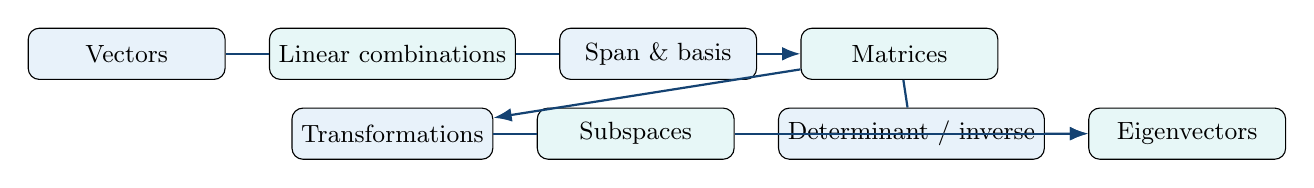
\begin{tikzpicture}[node distance=.35cm and .55cm, every node/.style={font=\small}]
\node[draw,rounded corners,fill=softblue,minimum width=2.5cm,minimum height=.65cm] (v) {Vectors};
\node[draw,rounded corners,fill=softteal,minimum width=2.5cm,minimum height=.65cm,right=of v] (lc) {Linear combinations};
\node[draw,rounded corners,fill=softblue,minimum width=2.5cm,minimum height=.65cm,right=of lc] (sp) {Span \& basis};
\node[draw,rounded corners,fill=softteal,minimum width=2.5cm,minimum height=.65cm,right=of sp] (m) {Matrices};
\node[draw,rounded corners,fill=softblue,minimum width=2.5cm,minimum height=.65cm,below=of lc] (t) {Transformations};
\node[draw,rounded corners,fill=softteal,minimum width=2.5cm,minimum height=.65cm,right=of t] (s) {Subspaces};
\node[draw,rounded corners,fill=softblue,minimum width=2.5cm,minimum height=.65cm,right=of s] (d) {Determinant / inverse};
\node[draw,rounded corners,fill=softteal,minimum width=2.5cm,minimum height=.65cm,right=of d] (e) {Eigenvectors};
\draw[-{Latex},thick,cusatblue] (v)--(lc)--(sp)--(m);
\draw[-{Latex},thick,cusatblue] (m)--(t);
\draw[-{Latex},thick,cusatblue] (m)--(d)--(e);
\draw[-{Latex},thick,cusatblue] (t)--(s)--(e);
\end{tikzpicture}

\vspace{.6cm}
\Large
\textbf{Represent} $\rightarrow$ \textbf{Transform} $\rightarrow$
\textbf{Analyze} $\rightarrow$ \textbf{Interpret}
\end{center}
\end{frame}

\begin{frame}{References and syllabus alignment}
\small
\begin{itemize}
\item CUSAT, M.Tech. CSE (Artificial Intelligence and Software Engineering), 2025 programme structure.
\item Gilbert Strang, \emph{Introduction to Linear Algebra}.
\item David C. Lay, Steven R. Lay, Judi J. McDonald, \emph{Linear Algebra and Its Applications}.
\item Sheldon Axler, \emph{Linear Algebra Done Right}.
\end{itemize}
\vspace{.2cm}
\begin{block}{Scope}
This presentation is built directly around the supplied topic list:
vectors, coordinates, operations, linear combinations, span/basis, matrix composition, 3D transformations, determinant, inverse, column/null spaces, nonsquare transformations, dot/duality, cross products, Cramer's rule, change of basis, eigenvalues/eigenvectors, and vector spaces.
\end{block}
\vfill
\centering
\textcolor{cusatblue}{\textbf{End of Module}}
\end{frame}

\end{document}
